%%%%%%%%%%%%%%% Analysis & Benchmark  %%%%%%%%%%%%%%%%%%%%%%%%%%%%%%%%
\section{Benchmark Analysis}
In order to quantify the success of our efforts, we performed a scaling analysis 
using a python script to plot different use cases.   
The first case explored was done by holding the number of particles, 
the mean free path of the particle, and the volume of the mesh constant while changing 
the number of voxels. Figure \ref{compare1} show the results for this analysis. 

\begin{figure}[H]
 \begin{centering}
 \centering
 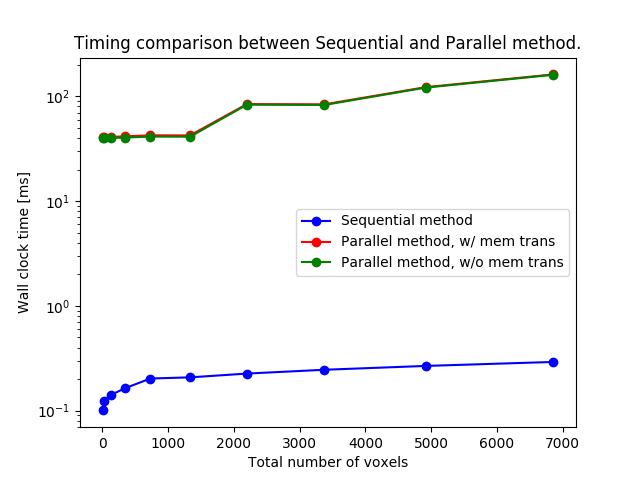
\includegraphics[width=0.6\linewidth,height=8cm]{../figs/compare.png}
 \caption{Comparison of sequential and parallel methods by changing the number of voxels}
 \label{compare1}
 \end{centering}
\end{figure}

In figure \ref{compare1}, we see that the sequential code runs faster than the 
parallel code. There are multiple explanation for this, but the most probably is the 
overheard related to memory access.

The second part of the analysis was done by using a mesh size with constant measurements 
and changing the mean free path of the particles. 


\begin{figure}[H]
 \begin{centering}
 \centering
 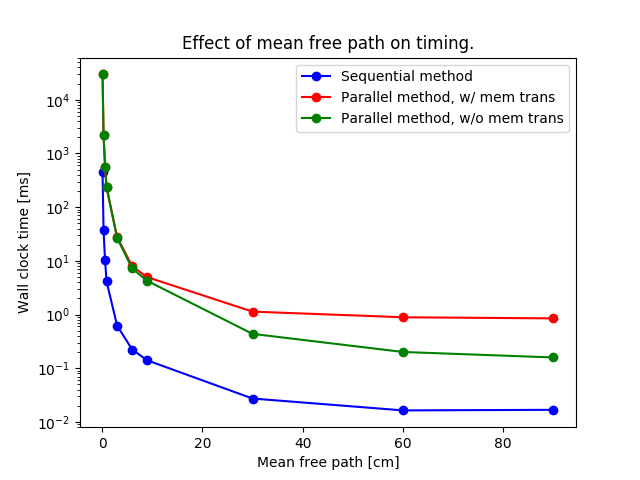
\includegraphics[width=0.6\linewidth,height=7cm]{../figs/mean_free_path.png}
 \caption{Comparison of sequential and parallel methods by changing the mean free path of the particle}
 \label{mean_free_path}
 \end{centering}
\end{figure}



The third scaling analysis was done using a mesh size with constant parameters and 
changing the number of particles run. Increasig the number of particles increases the 
number of tracks the code has to loop through. Figure \ref{particles} show the scaling results 
for this case. 
\begin{figure}[H]
 \begin{centering}
 \centering
 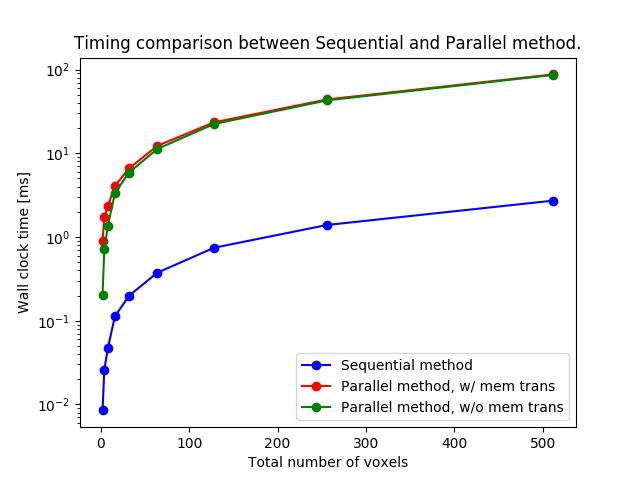
\includegraphics[width=0.6\linewidth,height=7cm]{../figs/particles.png}
 \caption{Comparison of sequential and parallel methods by changing the number of particles}
 \label{particles}
 \end{centering}
\end{figure}

